\chapter{Evaluation}
\label{ch:evaluation}
This chapter will cover the execution and evaluation of our benchmark with the workloads specified in section~\ref{ch:design:se:workloads}.
We will present the results of each workload and have a discussion on them directly after that.

A conclusion will be drawn in section~\ref{ch:futureWork:se:conclusion} in the next chapter.

\section{Objective}
The main goal is to see,
if the databases are capable of handling the production workloads.
To test that feature we will also make some other performance benchmarks to be able to evaluate the write speeds of the databases.

We want to measure the average time needed for a single insert operation,
that way we can compare the databases without take into account the overhead of the benchmark itself,
which will be reflected in the overall run time.

For the workloads including read operations we will also look at the overall run time to get a better view on the impact these operations have on the performance.

In section~\ref{ch:evaluation:se:overview} we will show which workloads we will compare with each other and what we want to evaluate through that comparison.

\section{Setup}
In this section we will describe the software and hardware we used to execute the benchmark.

\todo{explain how we evaluated the data, how executed? everything three times. Made average over results.}

\subsection{Hardware}
The computer used for the benchmark had the specifications shown in table~\ref{tab:hardware}.

\begin{table}[!h]
  \begin{minipage}{\textwidth}
    \begin{tabularx}{\textwidth}{ | l | X | }
      \hline
      Component & Description \\ \hline \hline
      CPU & Intel i7-3770K @ 3.5GHz \\ \hline
      RAM & 16GB DDR3 @ 1.600MHz \\ \hline
      Storage & Seagate ST2000DL003 2 TB 5900rpm, only a 400GB partition was used \\ \hline
      GPU & NVIDIA GeForce GTX 670 \\ \hline
    \end{tabularx}
  \end{minipage}
  \caption{The hardware specifications of the computer for the benchmark.}
  \label{tab:hardware}
\end{table}

\subsection{Software}
The versions of the software components we used are shown in the following table.

\begin{table}[h!]
  \begin{minipage}{\textwidth}
    \begin{tabularx}{\textwidth}{ | X | X | }
      \hline
      Software & Version \\ \hline \hline
      Ubuntu & 17.10 \\ \hline
      openjdk & xxx \\ \hline
      ssh & xxx \\ \hline
      YCSB & 0.14.0-SNAPSHOT \\ \hline
      ApacheJena & 3.6.0 \\ \hline
      Neo4j & 3.3.4 \\ \hline
      OrientDB & 2.2.33 \\ \hline
      Sparksee & 5.2.3 \\ \hline
    \end{tabularx}
  \end{minipage}
  \caption{The software specifications of the computer for the benchmark.}
  \label{tab:software}
\end{table}

\todo{the script, we stored histograms -> mean, stdD}

\section{Overview}
\label{ch:evaluation:se:overview}
\todo{Diagram to show the workflow of the script as the databases are used with the workloads, can be used for the presentation.}

The naming of the workloads is similar to the naming introduced in section~\ref{ch:design:se:workloads}.

\begin{landscape}
  \begin{table}
    \begin{minipage}{\hsize}
      \begin{tabularx}{\hsize}{ | l | l | l | l | X | }
        \hline
        Section & First workload & Other workload(s) & Units of measurement & Reason \\ \hline
        \ref{ch:evaluation:se:probingNodeCount} & 1. With Index & 2.-5. With Index & Inserts/second, total time, database size & The throughput in inserts/second will show if the databases slow down over time when they get filled up.
        The total time will show us,
        when the maximum dataset size is reached for each individual database in terms of reasonable execution time.\\ \hline
        \ref{ch:evaluation:se:probingNodeCount} & 1. Without Index & 2.-5. Without Index & Inserts/second & The throughput will show if the databases slow down as they get filled. \\ \hline
        \ref{ch:evaluation:se:probingNodeCount} & n.\footnote{the workload with the largest possible amount of nodes in terms of execution time.} With Index & n. Without Index & Inserts/second & To see how much time indexing takes up. \\ \hline
        \ref{ch:evaluation:se:probingNodeSize} & 1. Node Size & 2.-5. Node Size & Inserts/second, database size & We want to find the amount of data at which the databases are significantly slower.
        The database size of the different databases will show their storage efficiency. \\ \hline
        \ref{ch:evaluation:se:differenceEdges} & 1. No Edges & 2. No Edges & Inserts/second & Check if there is a benefit of an index if only nodes are inserted. \\ \hline
        \ref{ch:evaluation:se:differenceEdges} & n. With Index & 1. No Edges & Inserts/second & How much does inserting edges cost. \\ \hline
      \end{tabularx}
    \end{minipage}
    \caption{Overview for the throughput workloads}
    \label{tab:throughputOverview}
  \end{table}
  \begin{table}
    \begin{minipage}{\hsize}
      \begin{tabularx}{\hsize}{ | l | l | l | l | X | }
        \hline
        Section & First workload & Other workload(s) & Units of measurement & Reason \\ \hline
        \ref{ch:evaluation:se:productComplexity} & 1. Structure & 2.-3. Structure & Inserts/second & Does the structure has an impact on performance. \\ \hline
        \ref{ch:evaluation:se:productionSuitability} & x.\footnote{Every workload will be evaluated} Suitablitiy & - & Total time & Check if the workload is completed faster then the production period it represents. \\ \hline
        \ref{ch:evaluation:se:retrievingUnderLoad} & 1. Reading & 2. Reading & Reads/second & Observe if there is a difference in using an index. \\ \hline
        \ref{ch:evaluation:se:retrievingUnderLoad} & 1. Scanning & 2. Scanning & Scans/second & See if there is a difference in using an index for scanning. \\ \hline
        \ref{ch:evaluation:se:retrievingUnderLoad} & 1. Structure & 1. Reading \& Scanning & Operations/second & Investigate if other operations effect inserting data and compare operation throughput. \\ \hline
      \end{tabularx}
    \end{minipage}
    \caption{Overview for the production and retrieval workloads}
    \label{tab:productionOverview}
  \end{table}
\end{landscape}

\section{Throughput}
\todo{Tell at the beginning what we want to see.}
\label{ch:evaluation:se:throughput}
In this section we will examine the combinations of workloads mentioned in table~\ref{tab:throughputOverview}.
The results from these workloads will give us an understanding of how the databases perform in terms of insertions per seconds depending on different factors.

\subsection{Probing Node Count}
\label{ch:evaluation:se:probingNodeCount}
Here we will compare how the throughput, measured in inserts per second,
of the databases is effected by increasing the number of nodes we are inserting into it.

The throughput is listed in inserts per seconds,
which include both inserting nodes and inserting edges.

Apache Jena does not support indexing,
but it is still shown in most graphics as reference.

\subsubsection{Results}
The first figure~\ref{fig:withIndexThroughput} shows how the different databases perform with an increasing dataset size.
Apache Jena and Neo4j only have values for 1.000 and 10.000 nodes,
because execution with more than 10.000 nodes would take too much time.
Sparksee only delivered results up to 100.000 nodes,
because the free license only included database sizes of up to 1.000.000 elements and a workload with 1.000.000 nodes would contain 2.333.333 elements in total with the edges.

In figure~\ref{fig:withIndexExecutionTime} we see the execution time of the different databases.
At 10.000 nodes Apache Jena and Neo4j took almost an hour for one run,
because of that we did not run it with 100.000 nodes or more.

\begin{figure}[h!]
  \begin{minipage}{.5\textwidth}
    \centering
    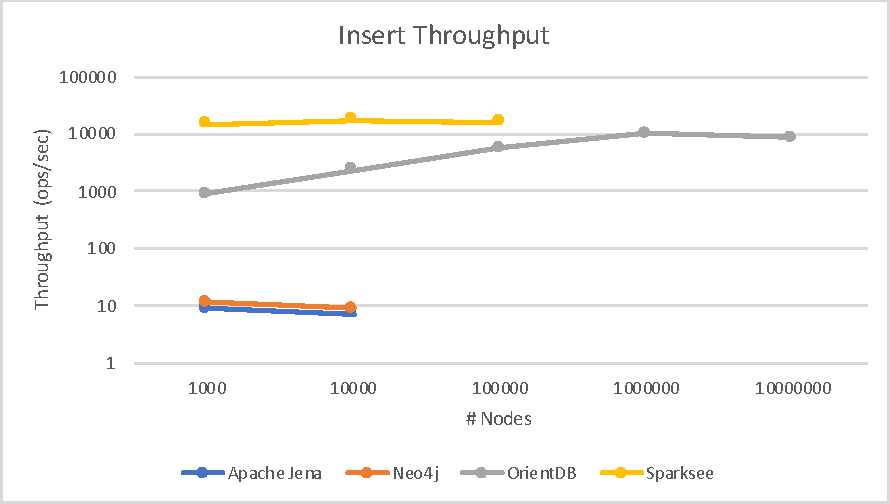
\includegraphics[width=\textwidth]{images/throughput/withIndexThroughput}
    \captionof{figure}{This figure shows the throughput in inserts/second of every database over different dataset sizes.}
    \label{fig:withIndexThroughput}
  \end{minipage}
  \begin{minipage}{.5\textwidth}
    \centering
    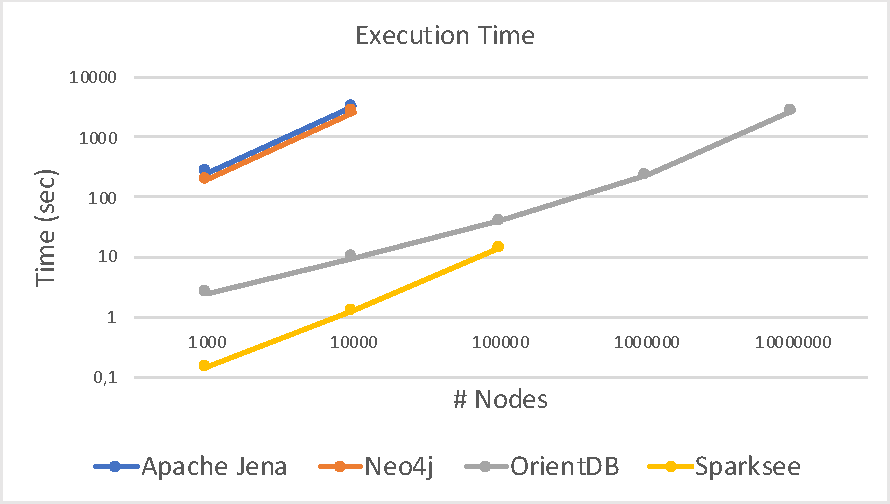
\includegraphics[width=\textwidth]{images/throughput/withIndexExecutionTime}
    \captionof{figure}{The execution time of the databases is shown over different dataset sizes.}
    \label{fig:withIndexExecutionTime}
  \end{minipage}
\end{figure}

Figure~\ref{fig:withoutIndexThroughput} shows the throughput over different dataset sizes without using an index.
In figure~\ref{fig:withWithoutIndexThroughputFixNodes} we see a comparison of using an index and not with a dataset size of 10.000 nodes.

\begin{figure}[h!]
  \begin{minipage}{.5\textwidth}
    \centering
    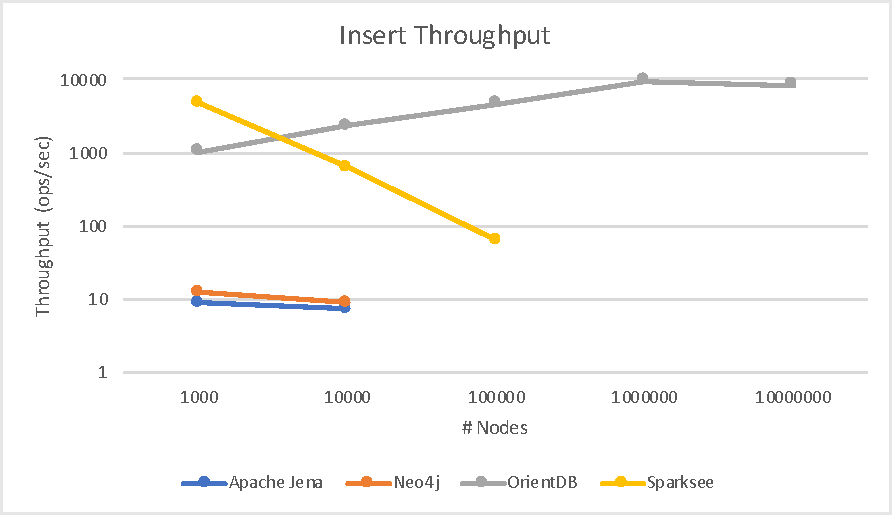
\includegraphics[width=\textwidth]{images/throughput/withoutIndexThroughput}
    \captionof{figure}{This diagram shows the throughput in inserts per second while using no index.}
    \label{fig:withoutIndexThroughput}
  \end{minipage}
  \begin{minipage}{.5\textwidth}
    \centering
    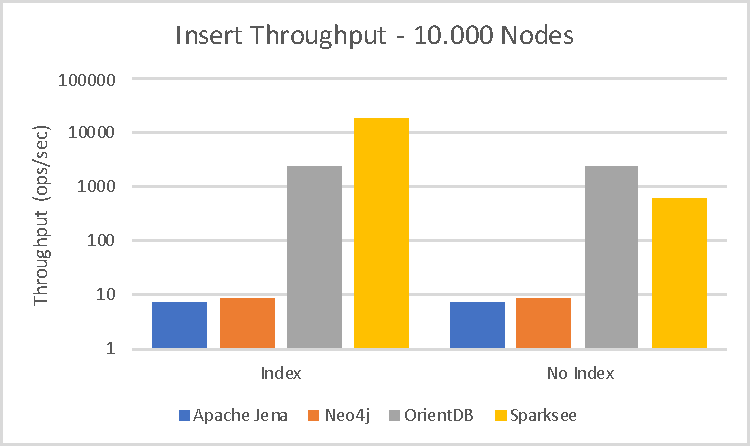
\includegraphics[width=\textwidth]{images/throughput/withWithoutIndexThroughputFixNodes}
    \captionof{figure}{The throughput at a fixed dataset size to compare between indexing and not.}
    \label{fig:withWithoutIndexThroughputFixNodes}
  \end{minipage}
\end{figure}

\subsubsection{Discussion}

\subsection{Probing Node Size}
\label{ch:evaluation:se:probingNodeSize}
In this subsection we will take a look at how the databases perform with different node property sizes.
We will pick a dataset size of 10.000 nodes,
as all database have a reasonable execution time with that amount of nodes.

\subsubsection{Results}
In figure~\ref{fig:nodeSize} we see,
how an increasing node size has an impact on insert throughput.

Figure~\ref{fig:sizeDatabaseSize} shows the size of the database folder,
in which the database stores its files.
The workload setup is the same as before.

\begin{figure}[h!]
  \begin{minipage}{.5\textwidth}
    \centering
    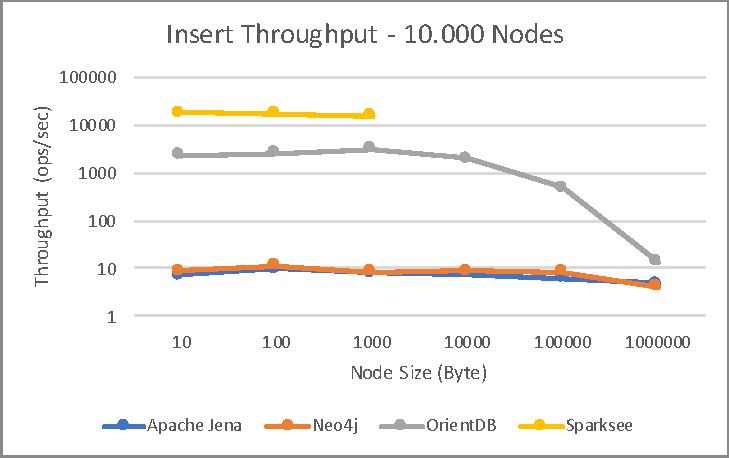
\includegraphics[width=\textwidth]{images/throughput/nodeSize}
    \captionof{figure}{Insert throughput over different node sizes with 10.000 nodes total.}
    \label{fig:nodeSize}
  \end{minipage}
  \begin{minipage}{.5\textwidth}
    \centering
    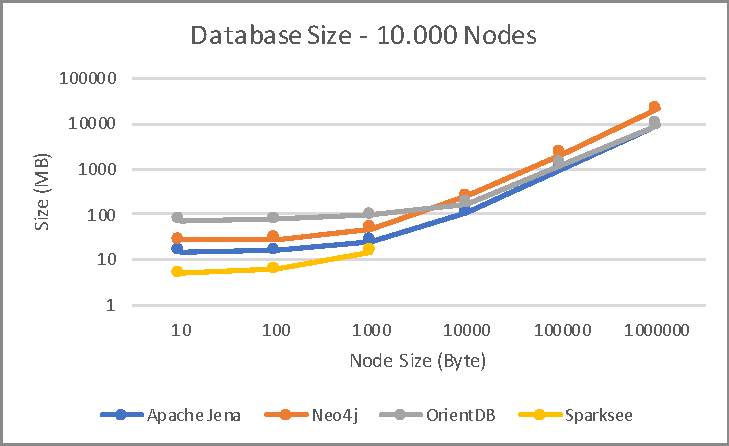
\includegraphics[width=\textwidth]{images/throughput/sizeDatabaseSize}
    \captionof{figure}{The size of the databases over growing node sizes.}
    \label{fig:sizeDatabaseSize}
  \end{minipage}
\end{figure}

\subsubsection{Discussion}

\subsection{Difference without Edges}
\label{ch:evaluation:se:differenceEdges}
Here we will investigate how the absents of edges has an impact on performance.
These workloads to not represent a real world scenario,
but they will provide us knowledge about how much inserting edges costs compared to nodes.

\subsubsection{Results}
Figure~\ref{fig:noEdges} shows us the difference in using an index compared to not doing so,
while only inserting nodes.

\begin{figure}[h!]
  \centering
  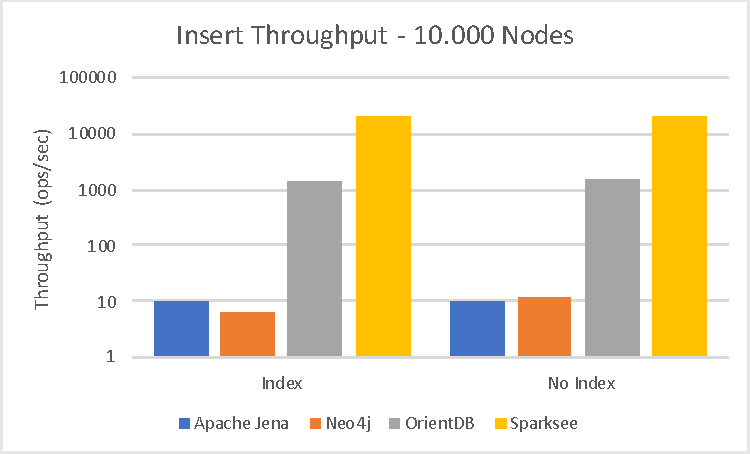
\includegraphics[width=.5\textwidth]{images/throughput/noEdges}
  \caption{Difference between using an index and not while using no edges.}
  \label{fig:noEdges}
\end{figure}

In figure~\ref{fig:indexNoEdges10000Nodes} we see a comparison of all databases between using edges and not with a dataset size of 10.000 nodes.
Figure~\ref{fig:indexNoEdges100000Nodes} shows a similar comparison with a bigger dataset,
but only between OrientDB and Sparksee,
as they were able to handle larger dataset within an acceptable time frame.

\begin{figure}[h!]
  \begin{minipage}{.5\textwidth}
    \centering
    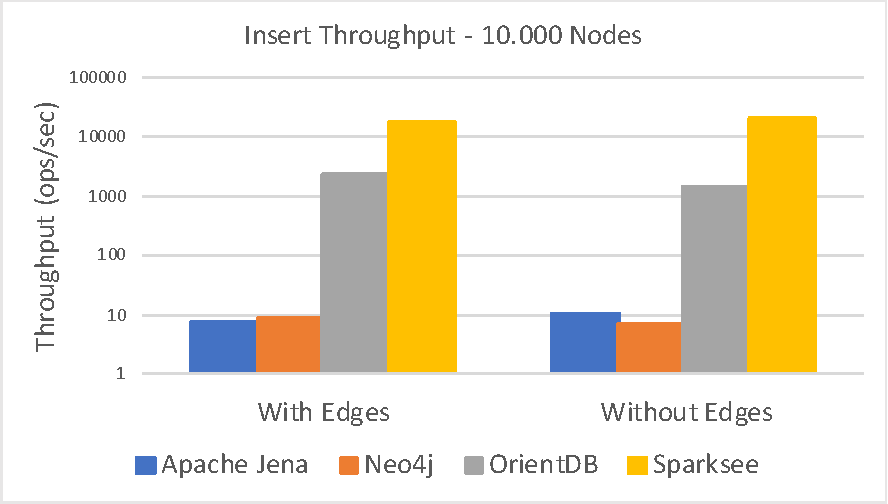
\includegraphics[width=\textwidth]{images/throughput/indexNoEdges10000Nodes}
    \captionof{figure}{Comparison of insert throughput between using edges and not.}
    \label{fig:indexNoEdges10000Nodes}
  \end{minipage}
  \begin{minipage}{.5\textwidth}
    \centering
    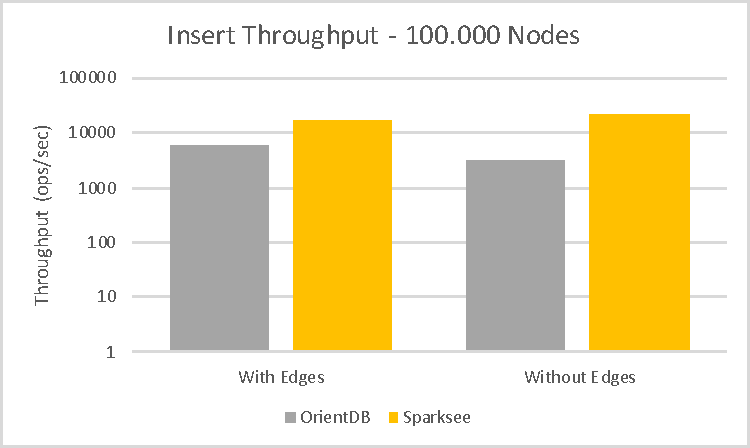
\includegraphics[width=\textwidth]{images/throughput/indexNoEdges100000Nodes}
    \captionof{figure}{Comparison with 100.000 nodes.}
    \label{fig:indexNoEdges100000Nodes}
  \end{minipage}
\end{figure}

\subsubsection{Discussion}

\section{Production Simulation}
\label{ch:evaluation:se:productionSimulation}
The workload results presented in this section will cover the production specific variables.
The first one being product complexity and the other one execution time.

\subsection{Product Complexity}
\label{ch:evaluation:se:productComplexity}
The product complexity describes,
how much the tree representing our data structure is widened at three different levels.

\subsubsection{Results}
In figure~\ref{fig:structure} we see the impact a different data structure has on the insert throughput.

\begin{figure}[h!]
  \centering
  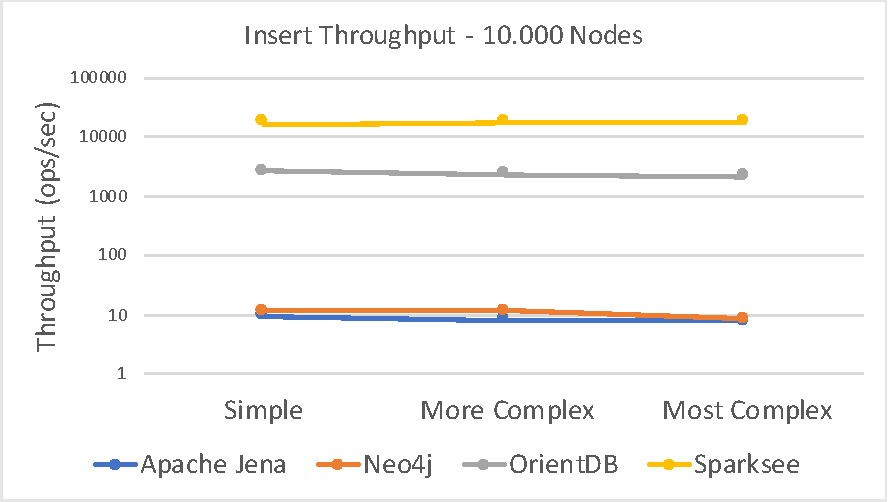
\includegraphics[width=.5\textwidth]{images/production/structure}
  \caption{Shows the difference in insert throughput over changing data structure.}
  \label{fig:structure}
\end{figure}

\subsubsection{Discussion}

\subsection{Production Suitability}
\label{ch:evaluation:se:productionSuitability}
The production simulations will finally show,
if the databases we chose are capable of storing the necessary amount of data in a specified time interval.

\subsubsection{Results}
Figure~\ref{fig:singleSuitability} show how long OrientDB took,
to store three minutes of production data (1.056.833 nodes).
Sparksee is mentioned with a theoretical time,
since it only allowed us to store 500.000 elements.
We took the throughput during inserting these 500.000 elements and calculated the time it would need to complete the whole workload.
The same was done for the results shown in figure~\ref{fig:hourSuitability}.

In figure~\ref{fig:hourSuitability} the same is shown but with a dataset that represents one hour of production,
which contains 21.136.660 nodes.

\begin{figure}[h!]
  \begin{minipage}{.5\textwidth}
    \centering
    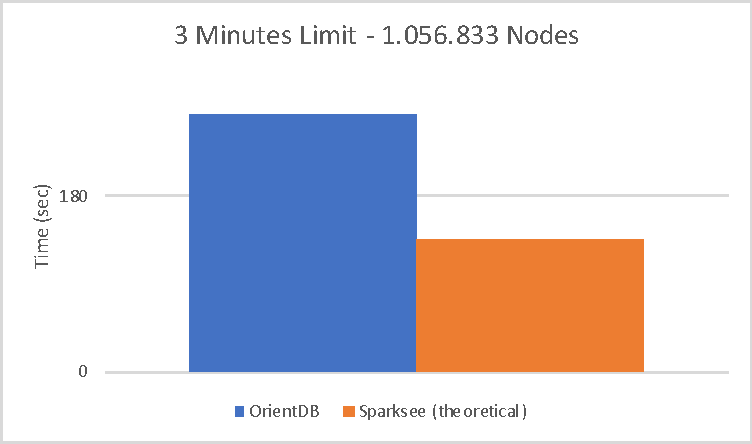
\includegraphics[width=\textwidth]{images/production/singleSuitability}
    \captionof{figure}{Shows the execution time with a dataset that represents three minutes of production.}
    \label{fig:singleSuitability}
  \end{minipage}
  \begin{minipage}{.5\textwidth}
    \centering
    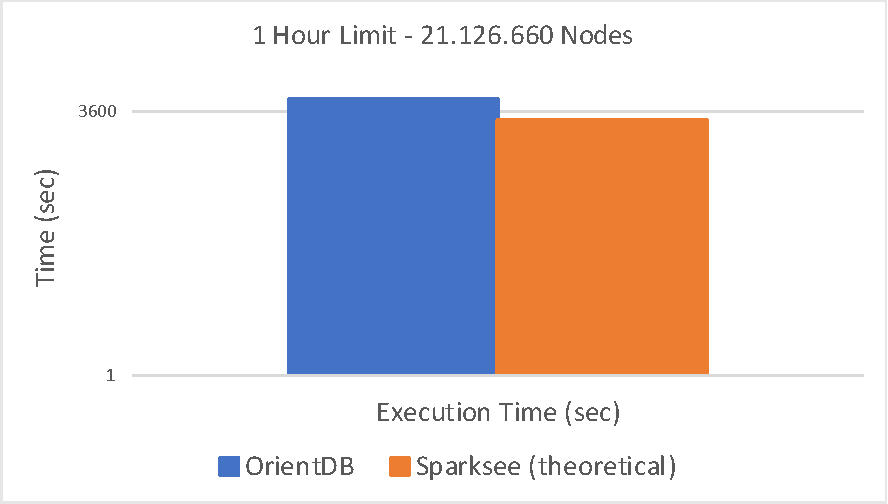
\includegraphics[width=\textwidth]{images/production/hourSuitability}
    \captionof{figure}{Shows the execution time with a dataset that represents one hour of production.}
    \label{fig:hourSuitability}
  \end{minipage}
\end{figure}

\subsubsection{Discussion}
\todo{Target throughput with total operations, see notes.md. Use to compare with workloads from above. With other structure we would need less...}

\section{Retrieving under load}
\label{ch:evaluation:se:retrievingUnderLoad}
This section will cover the results about retrieving data while the database is under load.
First we will take a look at how using an index is effecting the read and scan throughput,
then we will compare the throughput of the different operations~(\ref{fig:operationReadScan}) and their impact on the insert operation~(\ref{fig:insertWithWithoutReadScan}).

\subsection{Results}
In figure~\ref{fig:readThroughput10000Nodes} and~\ref{fig:scanThroughput10000Nodes} we see the throughput of read and scan operations when using an index or not.

\begin{figure}[h!]
  \begin{minipage}{.5\textwidth}
    \centering
    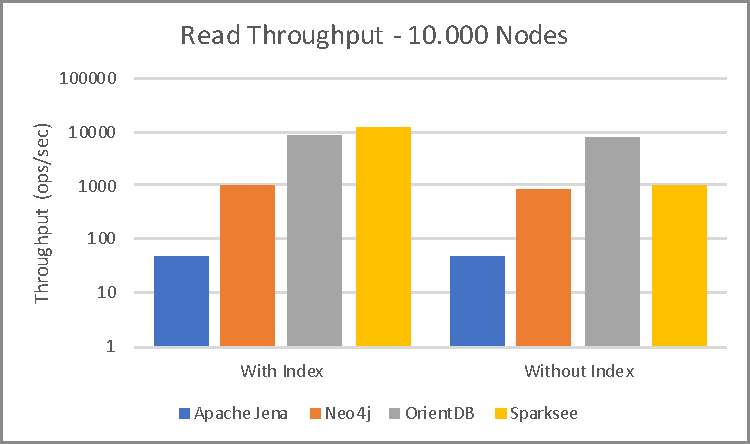
\includegraphics[width=\textwidth]{images/responsiveness/readThroughput10000Nodes}
    \captionof{figure}{Shows the throughput of read operations with and without the use of an index.}
    \label{fig:readThroughput10000Nodes}
  \end{minipage}
  \begin{minipage}{.5\textwidth}
    \centering
    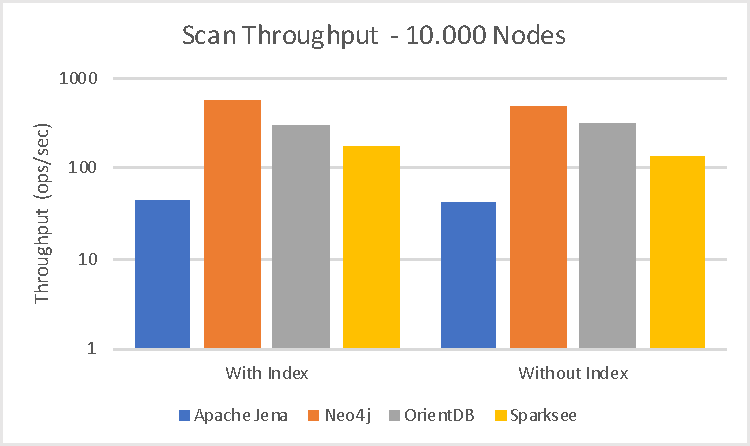
\includegraphics[width=\textwidth]{images/responsiveness/scanThroughput10000Nodes}
    \captionof{figure}{Shows the throughput of read operations with and without the use of an index.}
    \label{fig:scanThroughput10000Nodes}
  \end{minipage}
\end{figure}

Figure~\ref{fig:operationReadScan} shows the throughput of the different operations.
In figure~\ref{fig:insertWithWithoutReadScan} we see the impact of the read and scan operations on the insert operations.

\begin{figure}[h!]
  \begin{minipage}{.5\textwidth}
    \centering
    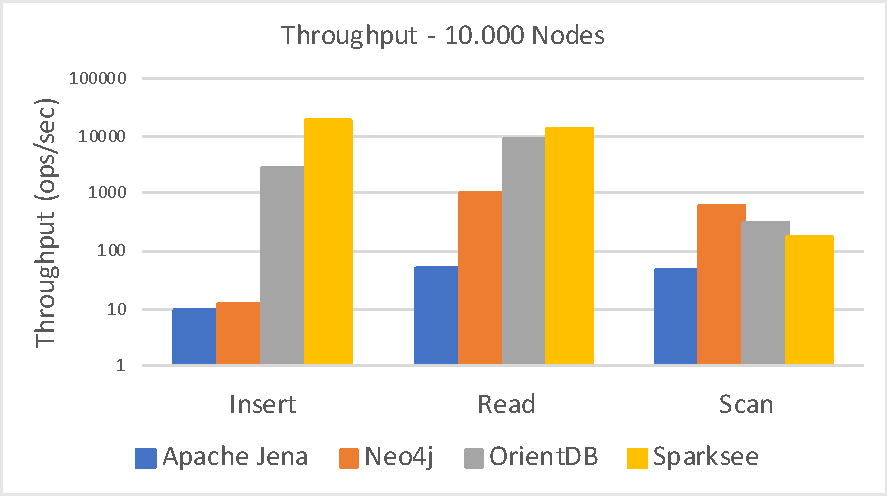
\includegraphics[width=\textwidth]{images/responsiveness/operationReadScan}
    \captionof{figure}{Shows the throughput of the different operations.\newline
    }
    \label{fig:operationReadScan}
  \end{minipage}
  \begin{minipage}{.5\textwidth}
    \centering
    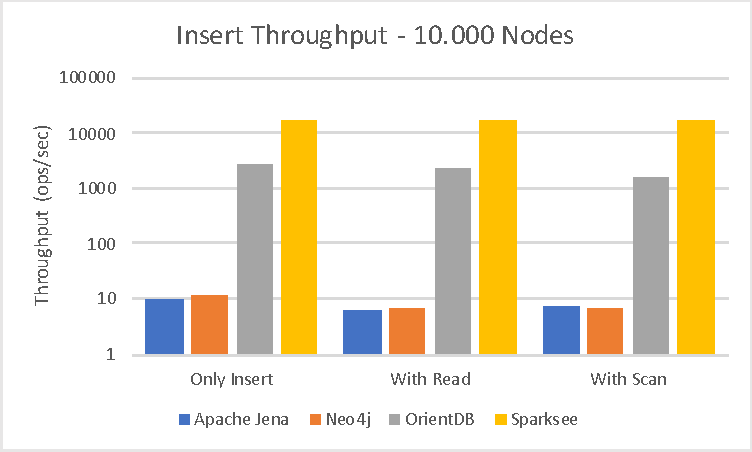
\includegraphics[width=\textwidth]{images/responsiveness/insertWithWithoutReadScan}
    \captionof{figure}{Shows the throughput of insert operations when using different operations.}
    \label{fig:insertWithWithoutReadScan}
  \end{minipage}
\end{figure}

\subsection{Discussion}
